\chapter{Realizacja projektu}
Niniejszy rozdział omówi architekturę i sposób implementacji projektu KubeFold.


\section{Koncepcja platformy KubeFold}
KubeFold to oprogramowanie, które działa na platformie Kubernetes w trybie Operatora.
Projekt składa się z następujących komponentów:
\begin{itemize}
    \item Operator Kubernetes (z ang. \textit{operator}) - komponent, który zarządzania logiką biznesową.
    Dba o poprawne uruchamianie i zarządzanie podami służącymi do pobierania baz danych białek oraz obliczeń.
    Komponent został dokładnie opisany w sekcji~\ref{subsec:component-operator}.
    \item Komponent pobierania (z ang. \textit{downloader}) - służy do kontroli procesu pobierania i dekompresji baz danych białek.
    Dokładny opis znajduje się w sekcji~\ref{subsec:component-downloader}.
    \item Komponent zarządzający obliczeniami (z ang. \textit{manager}) - obsługuje dodatkowe działania wokół obliczeń takie jak wysyłka artefaktów bądź wysyłanie powiadomienia.
    Opisany został w sekcji~\ref{subsec:component-manager}.
\end{itemize}

%TODO(matisiekpl): verify translation of CRD
Oprócz tego KubeFold wprowadza dwie CRD (\textit{custom resource definition}). Pierwszą z nich jest zasób $ProteinDatabase$.
Reprezentuje on pojedynczą instalację bazy danych białek w klastrze.
Przykładowy kod zasobu jest przedstawiony na listingu~\ref{lst:protein_database}.
W specyfikacji zasobów użytkownik może wybrać jakie bazy danych powinny zostać zainstalowane.
Co więcej, może też wskazać, jaką StorageClasse powinien przyjąć wolumen, służący do przechowywania danych.
Dzięki temu możliwe jest wskazanie klasy, która odpowiada za system plików Lustre (szerzej opisany w sekcji~\ref{subsec:lustre-volumes}).
W przykładowym kodzie wskazano klasę o nazwie \textit{fsx-sc}, która podpina się pod wolumeny AWS FSx for Lustre (zobacz~\ref{subsec:amazon-fsx-for-lustre}).

\begin{lstlisting}[language=yaml,caption={Przykładowy kod YAML zasobu ProteinDatabase},label={lst:protein_database}]
apiVersion: data.kubefold.io/v1
kind: ProteinDatabase
metadata:
  name: proteindatabase-sample
spec:
  datasets:
    bfd: true
    mgyclusters: true
    nt: true
    pdb: true
    pdbseqreq: true
    rfam: true
    rnacentral: true
    uniref90: true
    uniprot: true
  volume:
    storageClassName: fsx-sc
\end{lstlisting}

Ponadto KubeFold obsługuje definicję zasobu $ProteinConformationPrediction$.
Odpowiada on za pojedyncze obliczenie konformacji białka na podstawie dostarczonej sekwencji aminokwasów.
Przykład definicji jest przedstawiony na listingu~\ref{lst:protein_conformation_prediction}.
Użytkownik może wskazać ustawienia zadania takie jak:
\begin{itemize}
    \item bazę danych białek, na podstawie której algorytm AlphaFold ma przeprowadzić przeszukiwanie
    \item sekwencję aminokwasów w postaci ciągu liter
    \item ustawienia wolumenu służącego do przechowywania tymczasowych plików obliczenia
    \item wskazanie źródła pliku wag modelu AlphaFold.
    W przykładowym kodzie ustawiono źródło jako zdalny serwer HTTP.
    \item docelową lokalizację artefaktów.
    W aktualnej wersji projektu KubeFold wspierany jest jedynie system składowania obiektów AWS S3 (zobacz.~\ref{subsec:amazon-s3-object-storage}).
    \item opcje powiadamiania użytkownika.
    Przykładowy kod ma ustawione pojedyczne powiadomienie SMS na numer telefonu.
\end{itemize}

\begin{lstlisting}[language=yaml,caption={Przykładowy kod YAML zasobu ProteinConformationPrediction},label={lst:protein_conformation_prediction}]
apiVersion: data.kubefold.io/v1
kind: ProteinConformationPrediction
metadata:
  name: proteinconformationprediction-sample
spec:
  database: proteindatabase-sample
  protein:
    id: [ 'A','B' ]
    sequence: GMRESY...LQQANDLKQG
  model:
    volume:
      storageClassName: fsx-sc
    weights:
      http: https://staticfilehosting.com/af3.bin.zst
    seeds:
      - 1
  destination:
    s3:
      bucket: kubefold-artifacts-sample
      region: eu-central-1
  notify:
    region: eu-central-1
    sms:
      - "+48140690323"
\end{lstlisting}


\section{Użyte technologie}
Wszystkie trzy komponenty zostały napisane w języku Go w wersji 1.24 (więcej o nim w sekcji~\ref{subsec:go-programming-language}).
Był to naturalny wybór, ponieważ Go jest de facto standardem w przypadku tworzenia oprogramowania chmurowego.
Kod źródłowy komponentów był archiwizowany w repozytorium Git~\cite{git} w serwisie GitHub~\cite{github}.

W celu kompilacji aplikacji i spakowania plików wykonywalnych do obrazu kontenera użyto standardowego buildera od Dockera.

Dystrybucja obrazów odbywa się za pomocą rejestru Github Container Registry (\textit{ghcr.io})~\cite{ghcr}.
Obrazy są automatycznie budowane przy każdym wypchnięciu tagu Git przez narzędzie GitHub Actions~\cite{github_actions}.
Flow działania zostało przestawione na rys.~\ref{fig:docker-images-flow}.

\begin{figure}[htbp]
    \centering
    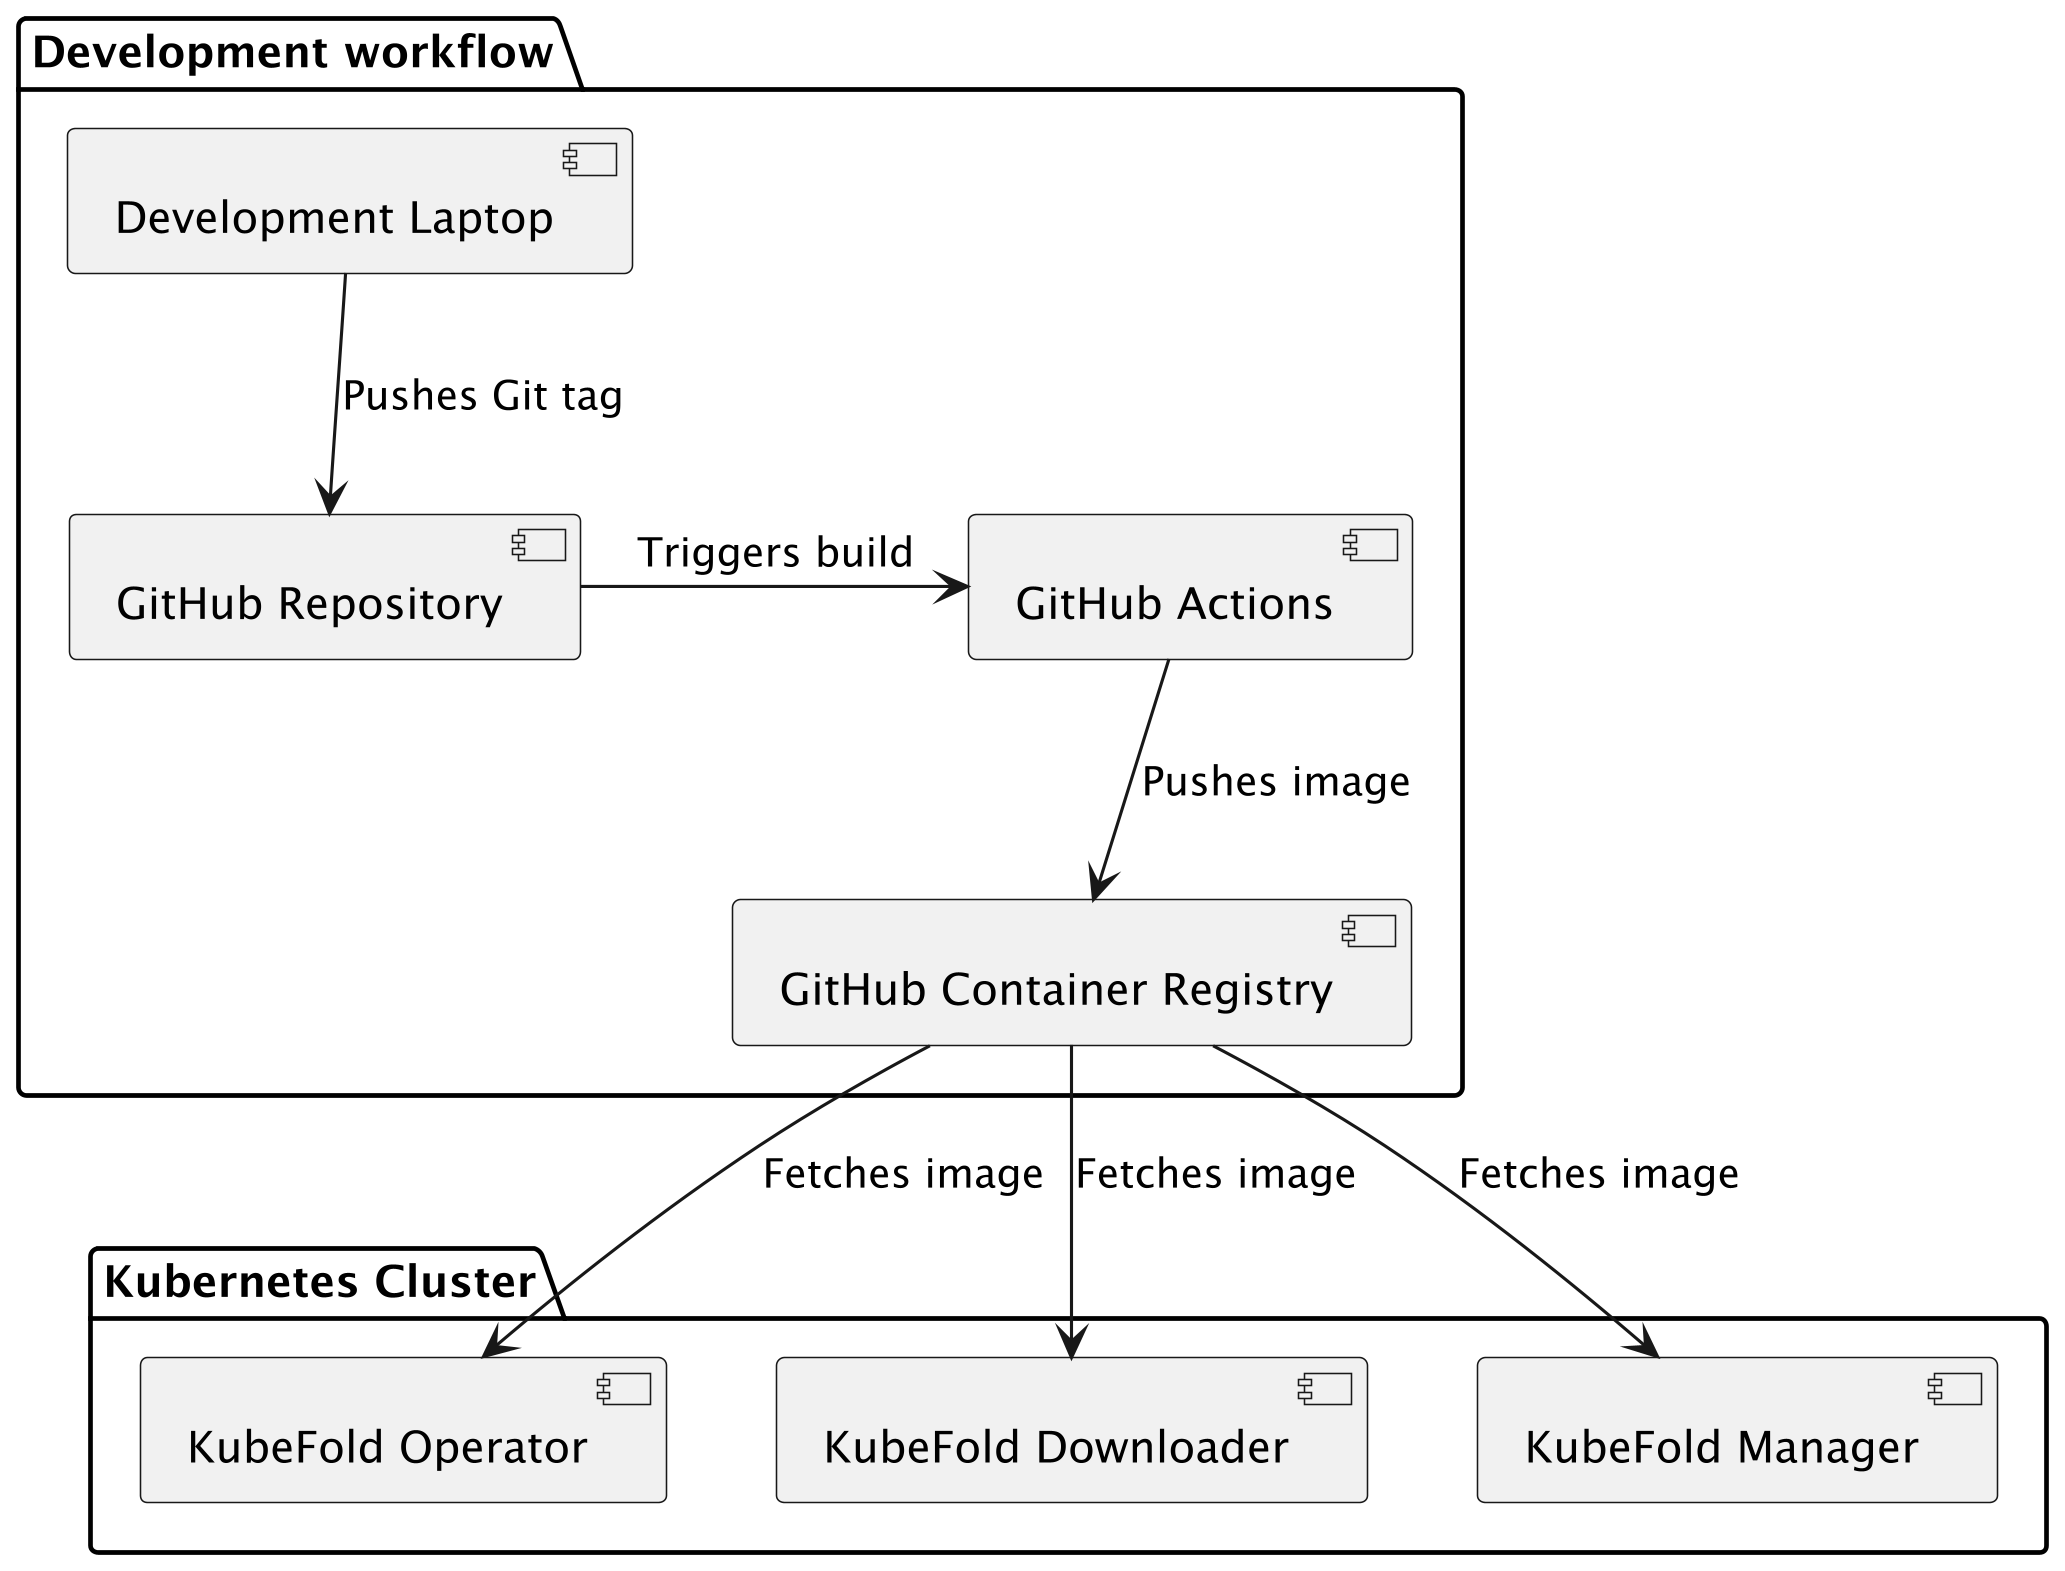
\includegraphics[width=0.8\textwidth]{images/images}
    \caption{Development workflow between GitHub and cluster}
    \label{fig:docker-images-flow}
\end{figure}

Komponent Operatora (szerzej opisany w~\ref{subsec:component-operator}) został utworzony na podstawie framework KubeBuilder~\cite{kubebuilder}.
KubeBuilder to framework, który służy do pisania natywnych operatorów Kubernetes.
Tworzy on strukturę katalogów projektu oraz od razu zapewnia zarządzanie elementami takimi jak:
\begin{itemize}
    \item Elekcja lidera operatora-niektóre instancje operatorów mogą być uruchomione na wielu węzłach klastra jednocześnie, aczkolwiek jeżeli istnieje potrzeba wybrania jednej wyróżnionej instancji, to elekcja lidera wybiera go.
    \item Generowanie skryptów instalacyjnych-KubeBuilder ma możliwość wygenerowania gotowych skryptów instalacyjnych, które mogą później posłużyć do automatycznej instalacji operatora i wszystkich jego zależności w klastrze jednym wykonaniem polecenia \textit{kubectl apply}.
    \item Definicje ról i permisji.
    Kubernetes korzysta z modelu autoryzacji o nazwie \textit{RBAC} (Role-Based Access Control)~\cite{k8s_rbac}.
    KubeBuilder wykrywa jakie permisje powinna mieć instancja operatora i upewnia się, że odpowiednie permisje zostały mu przyznane.
\end{itemize}


\section{Architektura rozwiązania}


\section{Opis komponentów}

\subsection{Komponent operatora}\label{subsec:component-operator}

\subsection{Komponent pobierania}\label{subsec:component-downloader}

\subsection{Komponent zarządzający obliczeniami}\label{subsec:component-manager}